%GiG
\documentclass{beamer} 
\usetheme{Copenhagen}
\setbeamertemplate{navigation symbols}{}
\setbeamertemplate{headline}{}
\DeclareMathOperator*{\argmax}{arg\,max}

\usepackage{hyperref}
\definecolor{azure}{rgb}{0.0, 0.5, 1.0}
%\newcommand{\tblue}[1]{\textcolor{blue}{#1}}
\newcommand{\tblue}[1]{{\Large {\textcolor{azure}{#1}}}}
\newcommand{\hred}[1]{{\textcolor{red}{#1}}}

\title[Saravanan Thirumuruganathan] 
{Lecture 1: Asymptotics, Recurrences, Elementary Sorting}

\author[CSE 5311] 
{Instructor: Saravanan Thirumuruganathan}

\date[] 

\begin{document}

\begin{frame}
  \titlepage
\end{frame}

%\begin{frame}{Outline}
%  \tableofcontents
%  % You might wish to add the option [pausesections]
%\end{frame}

\section{Outline}

\begin{frame}
\frametitle {Outline}
\begin{enumerate}
\item Introduction to Asymptotic Analysis
\begin{itemize}
\item Rate of growth of functions
\item Comparing and bounding functions: $O, \Theta, \Omega$
\item Specifying running time through recurrences
\item Solving recurrences
\end{itemize}
\item Elementary Sorting Algorithms
\begin{itemize}
\item Bubble, Insertion and Selection sort
\item Stability of sorting algorithms
\end{itemize}
\end{enumerate}
\end{frame}

\begin{frame}{In-Class Quizzes}
\begin{itemize}
\item {\Large {\bf URL:}} {\LARGE \bf \url{http://m.socrative.com/}} 
\item {\Large {\bf Room Name:} {\LARGE \bf 4f2bb99e}}
\end{itemize}
\end{frame}

\section{Analyzing Algorithms}
\begin{frame}{Analyzing Algorithms}

\tblue{Time Complexity:}
\begin{itemize}
\item Quantifies amount of \textbf{\textit{time}} an algorithm needs to complete as a {\em function} of input size
\end{itemize}
~\\
\tblue{Space Complexity:}
\begin{itemize}
\item Quantifies amount of \textbf{\textit{space}} an algorithm needs to complete as a {\em function} of input size
\end{itemize}
~\\
Function: Input size Vs \{Time, Space\}
\end{frame}

\begin{frame}{Analyzing Algorithms}

\tblue{Best Case Complexity:}
\begin{itemize}
\item of an algorithm is the {\bf function} that determines the {\bf minimum} number of steps taken on any problem instance of size $n$
\end{itemize}
\tblue{Worst Case Complexity:}
\begin{itemize}
\item $\ldots$ {\bf maximum} $\ldots$
\end{itemize}
\tblue{Average Case Complexity:}
\begin{itemize}
\item $\ldots$ {\bf average} $\ldots$
\end{itemize}
~\\
Function: Input size Vs \{Time, Space\}
\end{frame}

\begin{frame}{Rate of Growth of Functions}

\tblue{Growth Function $T(n)$}
\begin{itemize}
\item Input is positive integers $n=1,2,3, \ldots$
\item Asymptotically positive (returns positive numbers for large $n$)
\item How does $T(n)$ grow when $n$ grows?
\item $n$ is size of input
\item $T(n)$ is the amount of time it takes for an algorithm to solve some problem
\end{itemize}
\end{frame}


\begin{frame}{Rate of Growth of Functions}
\begin{center}
    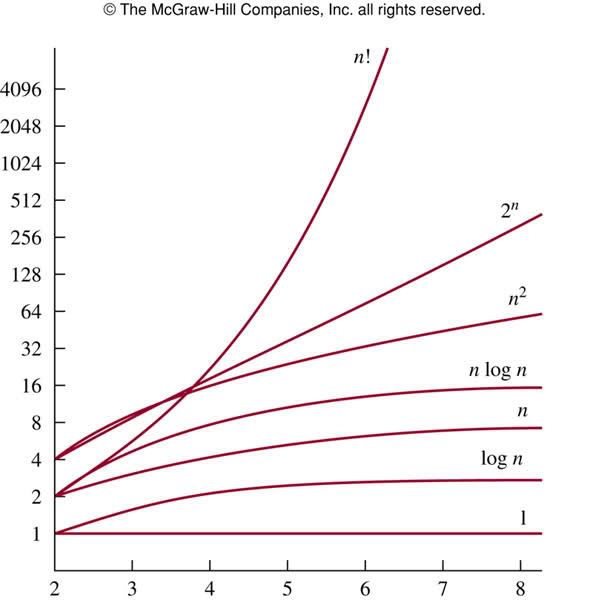
\includegraphics[scale=0.3]{rateOfGrowth.jpg}
\end{center}
\end{frame}

\begin{frame}{Quiz!}

\tblue{Question:}
\begin{itemize}
\item You have a machine that can do million operations per second.
\item Your algorithm requires $n^2$ steps
\item Suppose size of input is 1 million
\item How long does the algorithm takes for this input?
\end{itemize}
\end{frame}


\begin{frame}{Quiz!}

\tblue{Answer:}
\begin{itemize}
\item Algorithm will take $(1M)^2$ operations
\item Machine can do $1M$ operations per second
\item Running time = $\frac{(1M)^2}{1M}$ = $1M$ seconds
\item $1M$ seconds = $\frac{1M}{60*60*24}$ = Approximately $12$ days
\end{itemize}
\end{frame}


\begin{frame}{Why does it matter?}
Running time of different algorithms for various input sizes
\begin{center}
    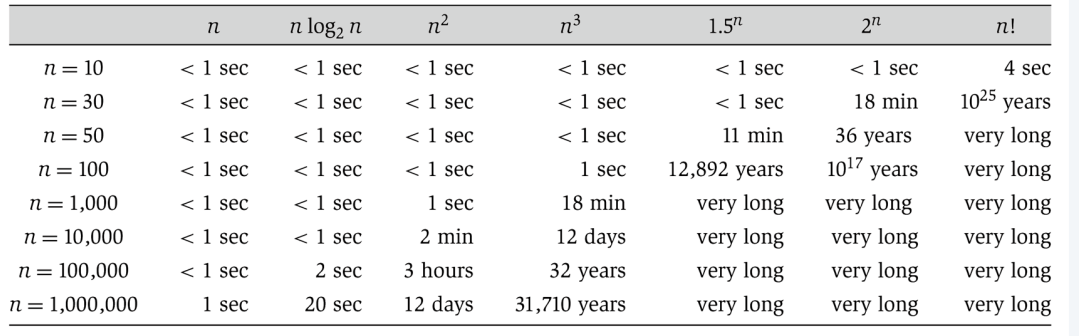
\includegraphics[scale=0.35]{fnVsTime.png}\footnote{Table 2.1 from K\&T Algorithm Design. Very long means it takes more than $10^{25}$ years.}
\end{center}
\end{frame}

\begin{frame}{Why does it matter?}
\begin{itemize}
\item The ``Big Data'' era
\item Can Google/Facebook/$\ldots$ use it?
\end{itemize}
\end{frame}


\begin{frame}{Functions in Real World}
This is how functions look in the real world!\footnote{Skiena Lecture notes}
\begin{center}
    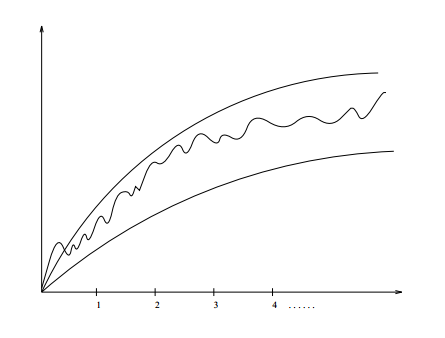
\includegraphics[scale=0.4]{realWorldFunctions.png}
\end{center}
\end{frame}


\begin{frame}{Solution: Analyze Asymptotic Behavior}
\begin{itemize}
\item Analyze the asymptotic behavior of algorithms
\item What happens to $f(n)$ when $n \to \infty$?
\end{itemize}
\begin{center}
\begin{table}[h]
\begin{tabular}{|c|c|c|}
\hline
       & $T(n)=1000n$ & $T(n)=n^2$       \\ \hline
$n=10$   & $10K$          & $100$        \\ \hline
$n=100$  & $100K$         & $10K$        \\ \hline
$n=1000$ & $1M$           & $1M$         \\ \hline
$n=10K$  & $10M$          & $100M$       \\ \hline
$n=100K$  & $100M$          & $10B$       \\ \hline
\end{tabular}
\end{table}
\end{center}
\end{frame}

\begin{frame}{Solution: Bound the functions}
\begin{itemize}
\item Identify known functions (such as $n, n^2, n^3, 2^n, \ldots$) that can ``bound'' $T(n)$
\item How to bound? - asymptotic {\bf upper, lower} and {\bf tight} bounds
\item Find a function $f(n)$ such that $T(n)$ is {\bf proportional} to $f(n)$
\item Why proportional (as against {\bf equal})?
\item Ignore aspects such as programming language, programmer capability, compiler optimization, machine specification etc
\end{itemize}
\begin{center}
    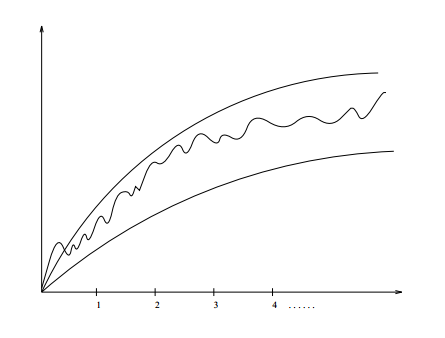
\includegraphics[scale=0.4]{realWorldFunctions.png}
\end{center}
\end{frame}


\begin{frame}{$O, \Omega, \Theta$\footnote{CLRS book}}
\begin{center}
    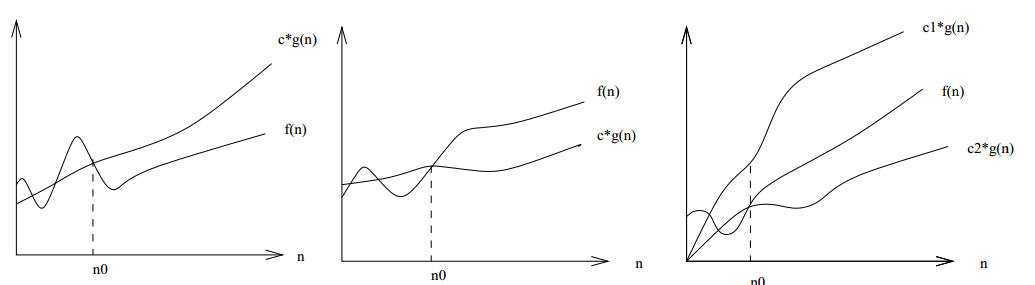
\includegraphics[scale=0.32]{allThreeBoundingFunctions.png}
\end{center}
\end{frame}

\begin{frame}{Big-O Notation}

\tblue{Upper bounds:} $T(n)$ is $O(f(n))$ if there exists {\bf constants} $c>0$ and $n_0 \geq 0$ such that
$T(n) \leq c \cdot f(n)$ for all $n \geq n_0$
\begin{center}
    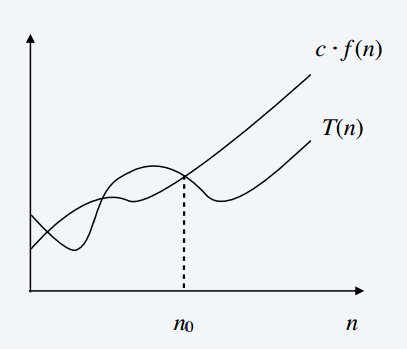
\includegraphics[scale=0.4]{bigOh.png}\footnote{From K\&T: Algorithm Design}
\end{center}
\end{frame}



\begin{frame}{Big-O Notation}

\tblue{Upper bounds:} $T(n)$ is $O(f(n))$ if there exists {\bf constants} $c>0$ and $n_0 \geq 0$ such that
$T(n) \leq c \cdot f(n)$ for all $n \geq n_0$

~\\
\textbf{Example:} $T(n)$ = $32n^2+17n+1$.  Is $T(n)$ in $O(n^2)$? 
\begin{itemize}
\item Yes! Use $c=50$, $n_0=1$
\item Simple Proof:
\end{itemize}
\begin{align*}
T(n) &\leq 32n^2+17n+1 \\
&\leq 32n^2+17n^2+1n^2 \\
&\leq 50n^2\\
&\leq cn^2\\
c=50    &   \text{ and } n_0=1
\end{align*}
Note: Not necessary to find the smallest $c$ or $n_0$
\end{frame}


\begin{frame}{Quiz!}
\textbf{Example:} $T(n)$ = $32n^2-17n+1$.  Is $T(n)$ in $O(n^2)$? 
\end{frame}

\begin{frame}{Big-O Notation}
\textbf{Example:} $T(n)$ = $32n^2-17n+1$.  Is $T(n)$ in $O(n^2)$? 
\begin{itemize}
\item Yes! Use $c=50$, $n_0=1$
\item Simple Proof:
\end{itemize}
\begin{align*}
T(n) &\leq 32n^2-17n+1 \\
&\leq 32n^2\textcolor{red}{+}17n+1 \\
&\leq 32n^2+17n^2+1n^2 \\
&\leq 50n^2\\
&\leq cn^2\\
c=50    &   \text{ and } n_0=1
\end{align*}
\end{frame}


\begin{frame}{Quiz!}
\textbf{Example:} $T(n)$ = $32n^2-17n+1$.  Is $T(n)$ in $O(n^3)$? 
\end{frame}

\begin{frame}{Big-O Notation}
\textbf{Example:} $T(n)$ = $32n^2-17n+1$.  Is $T(n)$ in $O(n^3)$? 
\begin{itemize}
\item Yes! Use $c=50$, $n_0=1$
\item Simple Proof:
\end{itemize}
\begin{align*}
T(n) &\leq 32n^2-17n+1 \\
&\leq 32n^2\textcolor{red}{+}17n+1 \\
&\leq 32n^2+17n^2+1n^2 \\
&\leq 50n^2\\
&\leq 50n^3\\
&\leq cn^3\\
c=50    &   \text{ and } n_0=1
\end{align*}
\end{frame}



\begin{frame}{Quiz!}
\textbf{Example:} $T(n)$ = $32n^2+17n+1$.  Is $T(n)$ in $O(n)$? 
\end{frame}

\begin{frame}{Big-O Notation}
\textbf{Example:} $T(n)$ = $32n^2+17n+1$.  Is $T(n)$ in $O(n)$? 
\begin{itemize}
\item No!
\item Proof by contradiction
\end{itemize}
\begin{align*}
32n^2+17n+1 &\leq c \cdot n\\
32n+17+\frac{1}{n} &\leq c \\
32n &\leq c \text{ (ignore constants for now)} \\
n &\leq c \text{ (ignore constants for now)} \\
\end{align*}
This inequality does not hold for $n=c+1$!
\end{frame}



\begin{frame}{Set Theoretic Perspective}
\begin{itemize}
\item $O(f(n))$ is set of all functions $T(n)$ where there exist positive constants $c, n_0$ 
such that $0 \leq T(n) \leq c \cdot f(n)$ for all $n \geq n_0$
\item Example: $O(n^2)=$ \{ $n^2, \ldots, 32n^2+17n+1$, $32n^2-17n+1$, $\ldots, n, 2n, \ldots $\}
\item Notation: $T(n)=O(f(n))$ or $T(n) \in O(f(n))$
\end{itemize}
\end{frame}


\begin{frame}{Limit based Perspective}
\begin{itemize}
\item $T(n)$ is $O(f(n))$ if $\limsup\limits_{n \rightarrow \infty} \frac{T(n)}{f(n)} < \infty$ 
\item Example: $32n^2+17n+1$ is $O(n^2)$
\end{itemize}
\begin{align*}
\limsup\limits_{n \rightarrow \infty} \frac{T(n)}{f(n)} &= \frac{32n^2+17n+1}{n^2} \\
&= 32 + \frac{17}{n} + \frac{1}{n^2} \\
&= 32 < \infty
\end{align*}
\end{frame}


\begin{frame}{Big-Omega Notation}

\tblue{Lower bounds:} $T(n)$ is $\hred{\Omega}(f(n))$ if there exists {\bf constants} $c>0$ and $n_0 \geq 0$ such that
$T(n) \hred{\geq} c \cdot f(n)$ for all $n \geq n_0$
\begin{center}
    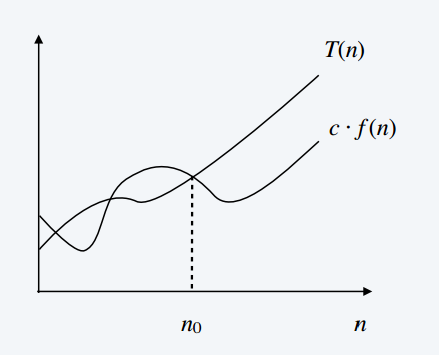
\includegraphics[scale=0.4]{bigOmega.png}\footnote{From K\&T: Algorithm Design}
\end{center}
\end{frame}


\begin{frame}{Big-Omega Notation}

\tblue{Lower bounds:} $T(n)$ is $\Omega(f(n))$ if there exists {\bf constants} $c>0$ and $n_0 \geq 0$ such that
$T(n) \geq c \cdot f(n)$ for all $n \geq n_0$

~\\
\textbf{Example:} $T(n)$ = $32n^2+17n+1$.  Is $T(n)$ in $\Omega(n^2)$? 
\begin{itemize}
\item Yes! Use $c=32$, $n_0=1$
\item Simple Proof:
\end{itemize}
\begin{align*}
T(n) &\geq 32n^2+17n+1 \\
&\geq 32n^2\\
&\geq cn^2\\
c=32    &   \text{ and } n_0=1
\end{align*}
\end{frame}


\begin{frame}{Big-Theta Notation}

\tblue{Tight bounds:} $T(n)$ is $\hred{\Theta}(f(n))$ if there exists {\bf constants} $\hred{c_1>0, c_2>0}$ and $n_0 \geq 0$ such that
\hred{$c_1 \cdot f(n) \leq T(n) \leq c_2 \cdot f(n)$} for all $n \geq n_0$
\begin{center}
    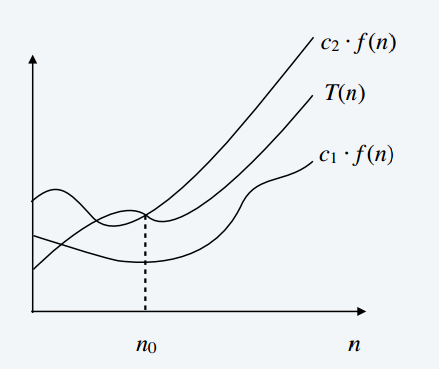
\includegraphics[scale=0.4]{bigTheta.png}\footnote{From K\&T: Algorithm Design}
\end{center}
\end{frame}


\begin{frame}{Big-Theta Notation}

\tblue{Tight bounds:} $T(n)$ is $\hred{\Theta}(f(n))$ if there exists {\bf constants} $\hred{c_1>0, c_2>0}$ and $n_0 \geq 0$ such that
\hred{$c_1 \cdot f(n) \leq T(n) \leq c_2 \cdot f(n)$} for all $n \geq n_0$

~\\
\textbf{Example:} $T(n)$ = $32n^2+17n+1$.  Is $T(n)$ in $\Omega(n^2)$? 
\begin{itemize}
\item Yes! Use $c_1=32$, $c_2=50$ and $n_0=1$
\item Combine proofs from before
\end{itemize}

~\\
{\bf Theorem:} For any two functions $f(n)$ and $g(n)$, we have $f(n) = \Theta(g(n))$ if and only if 
$f(n) = O(g(n))$ and $f(n)=\Omega(g(n))$ 
\end{frame}



\begin{frame}{Limit based Definitions}
Let $\limsup\limits_{n \rightarrow \infty} \frac{T(n)}{f(n)} = c$
\begin{itemize}
\item If $c < \infty$ then $T(n)$ is $O(f(n))$  (typically $c$ is zero)
\item If $c > 0$ then $T(n)$ is $\Theta(f(n))$  (also $O(f(n))$ and $\Omega(f(n))$)
\item If $c = \infty$ then $T(n)$ is $\Omega(f(n))$ 
\end{itemize}
\end{frame}

\begin{frame}{Some Big-O tips}
\begin{itemize}
\item Big-O is one of the most useful things you will learn in this class!
\item Big-O ignores {\em constant} factors through $c$ 
\begin{itemize}
\item Algorithm implemented in Python might need a larger $c$ than one implemented in C++
\end{itemize}
\item Big-O ignores small inputs through $n_0$ 
\begin{itemize}
\item Simply set a large value of $n_0$
\end{itemize}
\item Suppose $T(n)$ is $O(f(n))$. Typically, $T(n)$ is messy while $f(n)$ is simple 
\begin{itemize}
\item $T(n)=32n^2+17n+1$, $f(n)=n^2$
\end{itemize}
\item Big-O hides constant factors. Some times using an algorithm with worser Big-O might still be a good idea 
(e.g. sorting, finding medians)
\end{itemize}
\end{frame}

\begin{frame}{Survey of Running Times}
\begin{center}
    \begin{table}[h]
        \begin{tabular}{|l|l|p{2in}|}
            \hline
            {\bf Complexity} & {\bf Name} & {\bf Example} \\ \hline
            $O(1)$ & Constant time & Function that returns a constant (say 42)\\ \hline
            $O(\log n)$ & Logarithmic & Binary Search \\ \hline
            $O(n)$ & Linear & Finding Max of an array\\ \hline
            $O(n \log n)$ & Linearithmic & Sorting (for e.g. Mergesort) \\ \hline
            $O(n^2)$ & Quadratic & Selection sort \\ \hline
            $O(n^3)$ & Cubic & Floyd-Warshall \\ \hline
            $O(n^k)$ & Polynomial & Subset-sum with $k$ elements\\ \hline
            $O(2^n)$ & Exponential & Subset-sum with no cardinality constraints\\ \hline
        \end{tabular}
    \end{table}
\end{center}
\end{frame}


\begin{frame}{Dominance Rankings\footnote{Skiena lecture notes}}
\begin{itemize}
\item $n! \gg 2^n \gg n^3 \gg n^2 \gg n \log n \gg n \gg \log n \gg 1$
\item Exponential algorithms are useless even at $n >= 50$
\item Quadratic algorithms at around $n \geq 1M$
\item $O(n \log n)$ at around $n \geq 1B$
\end{itemize}
\end{frame}

\section{Recurrences}
\begin{frame}{Closer Look at $T(n)$}
\begin{itemize}
\item So far we assumed someone gave us $T(n)$ 
\item What is $n$? (Program Analysis)
\item How do we get $T(n)$? (Recurrences)
\end{itemize}
\end{frame}


\begin{frame}[fragile]{Program Analysis}
  \begin{columns}
    \begin{column}{0.5\textwidth}
\begin{verbatim}
for i=1 to n
{
    constant time
    operations
}
\end{verbatim}
    \end{column}
    \begin{column}{0.5\textwidth}
\begin{verbatim}
for i=1 to n
{
    for j=1 to n
    {
        constant time 
        operations 
    }
}
\end{verbatim}
    \end{column}
  \end{columns}
\end{frame}

\begin{frame}{Recurrences}
\begin{itemize}
\item Typically programs are lot more complex than that
\item Recurrences occur in recursion and divide and conquer paradigms
\item Specify running time as a function of $n$ and running time over inputs of smaller sizes
\item Examples:
\begin{itemize}
    \item fibonacci($n$) = fibonacci($n-1$) + fibonacci($n-2$)
    \item $T(n) = 2T(\frac{n}{2}) + n$
    \item $T(n) = T(n-1) + n$
\end{itemize}
\end{itemize}
\end{frame}


\begin{frame}{Solving Recurrences}
\begin{itemize}
\item Unrolling
\item Guess and prove by induction (aka Substitution)
\item Recursion tree
\item Master method
\end{itemize}
\end{frame}


\begin{frame}{Unrolling}
Let $T(n) = T(n-1) + n$. Base case: $T(1)=1$
\begin{align*}
T(n)    &= T(n-1) + n \\
        &= n + T(n-1) \\
        &= n + n-1 + T(n-2) \\
        &= n + n-1 + n-2 + T(n-3) \\
        &= n + n-1 + n-2 + n-3 + \ldots + 4 + 3 + 2 + 1 \\
        &= \frac{n(n-1)}{2} \\
        &= 0.5n^2 - 0.5n \\
        &= O(n^2)
\end{align*}
\end{frame}

\begin{frame}{Quiz!}
Solve $T(n) = 2T(n-1)$. Base case: $T(1)=1$ 
\end{frame}


\begin{frame}{Quiz!}
Solve $T(n) = 2T(n-1)$. Base case: $T(1)=1$ 
\begin{align*}
T(n)    &= 2T(n-1) \\
        &= 2( 2T(n-2) ) \\
        &= 2( 2( 2T(n-3))) \\
        &= 2^3 T(n-3) \\
        &= 2^i \ldots 2T(n-i) \\
        &= 2^n \\
        &= O(2^n)
\end{align*}
\end{frame}


\begin{frame}{Recursion Tree}
$T(n) = T(\frac{2n}{3}) + T(\frac{n}{3}) + cn$
\begin{center}
    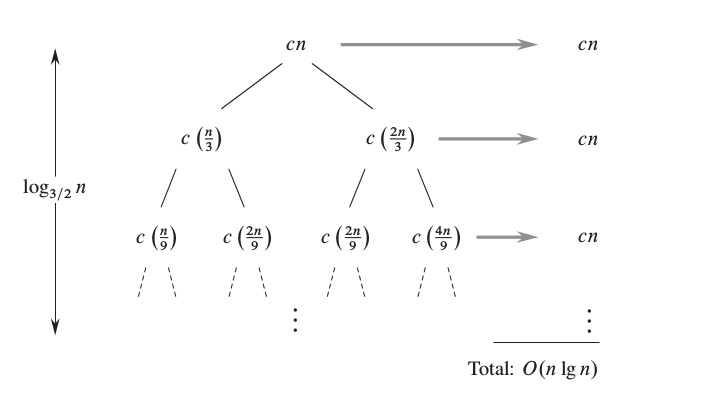
\includegraphics[scale=0.4]{recursionTree.png}\footnote{From CLRS}
\end{center}
\end{frame}

\begin{frame}{Logarithms\footnote{Skiena Lectures}}
\begin{itemize}
\item Logarithm is an {\em inverse} exponential function
\item $b^x = n$ implies $x=\log_b n$
\item If $b=2$, logarithms reflect how many times we can double something until we get $n$ or halve something till we get $1$
\item Example: $2^4=16$, $\log_2 16 = \hred{\lg } 16 = 4$
\item Example: You need $\lg 256 = 8$ bits to represent $[0,255]$
\item Identities:
\begin{itemize}
    \item $\log_b (xy) = \log_b (x) + \log_b(y)$
    \item $\log_b a = \frac{\log_c a}{\log_c b}$
    \item $\log_b b = 1$ and $\log_b 1 = 0$
\end{itemize}
\end{itemize}
\end{frame}


\end{document}

